\documentclass[12pt]{article} 
\usepackage[utf8]{inputenc}
\usepackage[T2A]{fontenc}
\usepackage{amsthm}
\usepackage{amssymb}
\usepackage{blindtext}
\usepackage{amsmath}
\usepackage{tikz} 
\usepackage{listings}
\usepackage{xcolor}
\usepackage{float}
\usepackage{graphicx}
\usepackage{hyperref}
\usepackage{wrapfig}
\hypersetup{
    colorlinks=true,
    linkcolor=blue,
    filecolor=blue,      
    urlcolor=blue,
    pdftitle={Overleaf Example},
    pdfpagemode=FullScreen,
    }
\graphicspath{ {./images} }

\title{Bioinformatics HW3}
\author{Ershov Ivan}
\date{December 2021}

\begin{document}
\maketitle
\paragraph{Задание 1.\\}
Я выбрал 9 геномов коронавируса людей из следующих стран:
\begin{enumerate}
    \itemsep0em
    \item Australia 
    \item Chine
    \item Czech Republic
    \item Egypt
    \item Germany
    \item Israel
    \item Italy
    \item Peru
    \item USA
\end{enumerate}
А также взял геном коронавируса SARS-CoV-1.\\
Теперь в программе MEGA выравняем эти последовательности при помощи алгоритма Muscle. После этого построим филогенетические деревья методом расстояний (Neighbor-Joining и UPGMA), методом максимального правдоподобия (Maximum Likelihood) и методом максимальной бережливости (Maximum Parsimony). Будем строить без бутстрэпа, так как он имеет смысл только при большом количестве мутаций.

\newpage
Будем считать суммы длин ветвей от SARS-CoV-1 до других геномов. Геномы коронавируса, которые расположены в дереве "дальше всего" от SARS-CoV-1, имеют больше всего мутаций относительно SARS-CoV-1, а значит, человек, из которого взяли образец генома данного коронавируса, был заражен позже всех. Аналогично: геном, который ближе к SARS-CoV-1, имеет меньше всего мутаций, а значит вирус заразил человека раньше остальных.

\subparagraph{Neighbor-Joining\\}
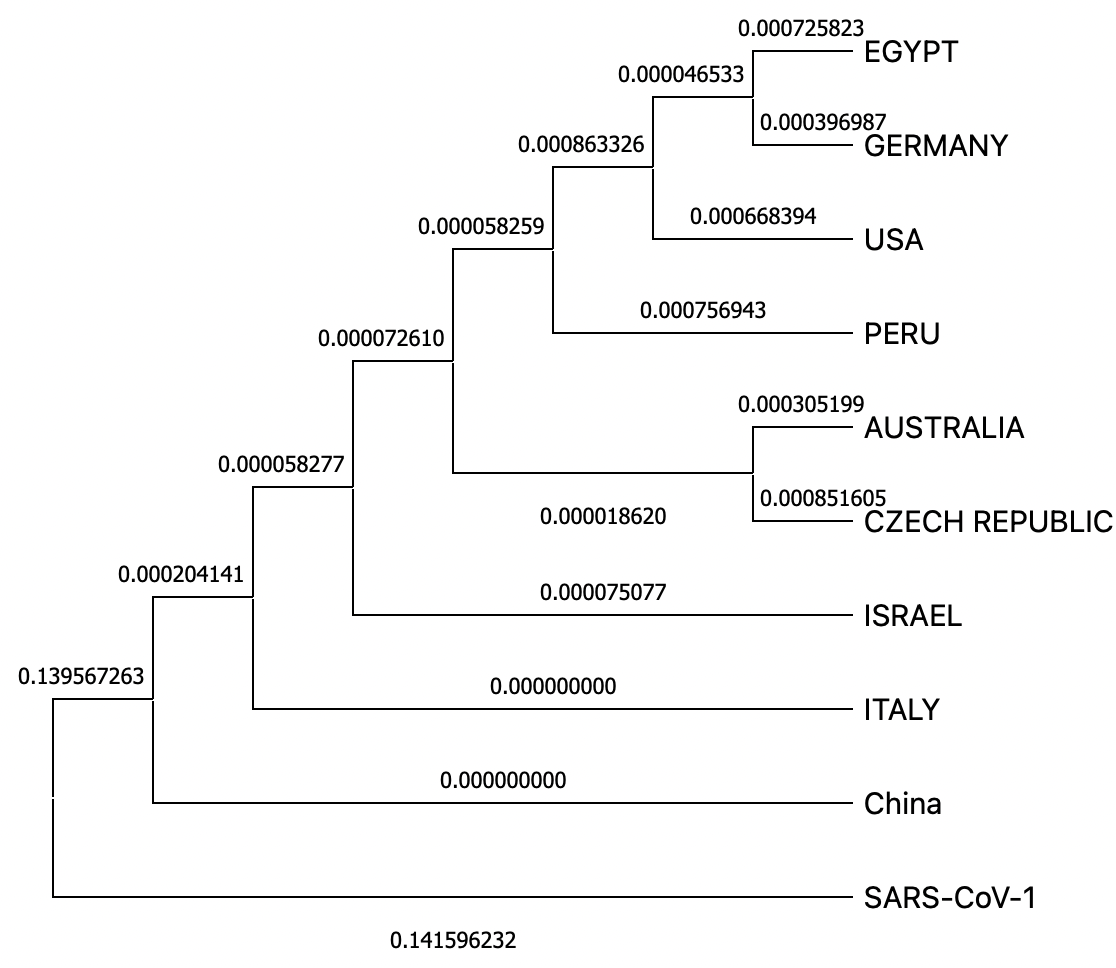
\includegraphics[scale=0.7]{images/NJ.png}\\

Заметим, что в данном случае самый ближайший геном\\к SARS-CoV-1 - это Chine, а самый дальний - Germany и Egypt

\subparagraph{UPGMA\\}
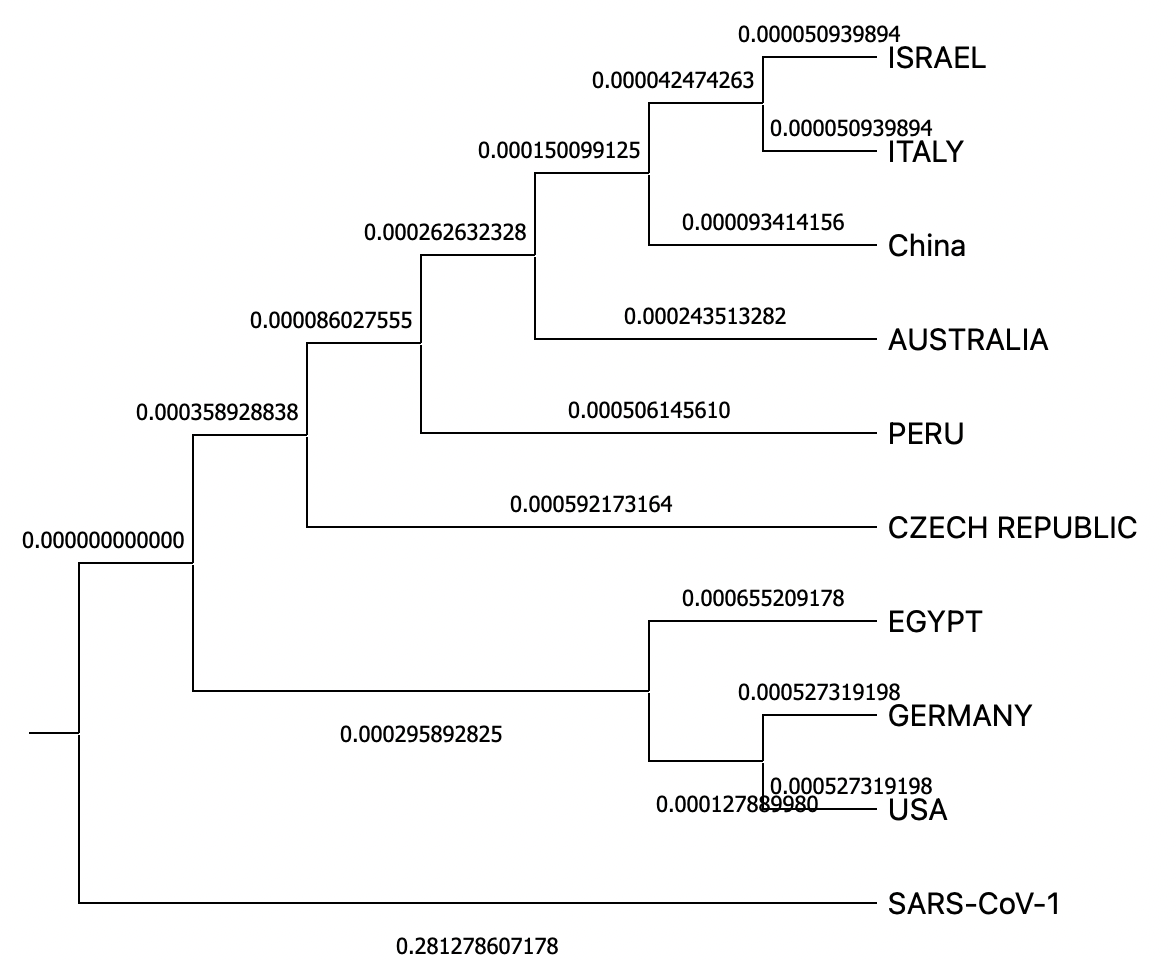
\includegraphics[scale=0.85]{images/UPGMA.png}\\

Заметим, что в данном случае самый ближайший геном\\к SARS-CoV-1 - это Chine, а самый дальний - Germany, USA и Egypt

\subparagraph{Maximum Likelihood\\}
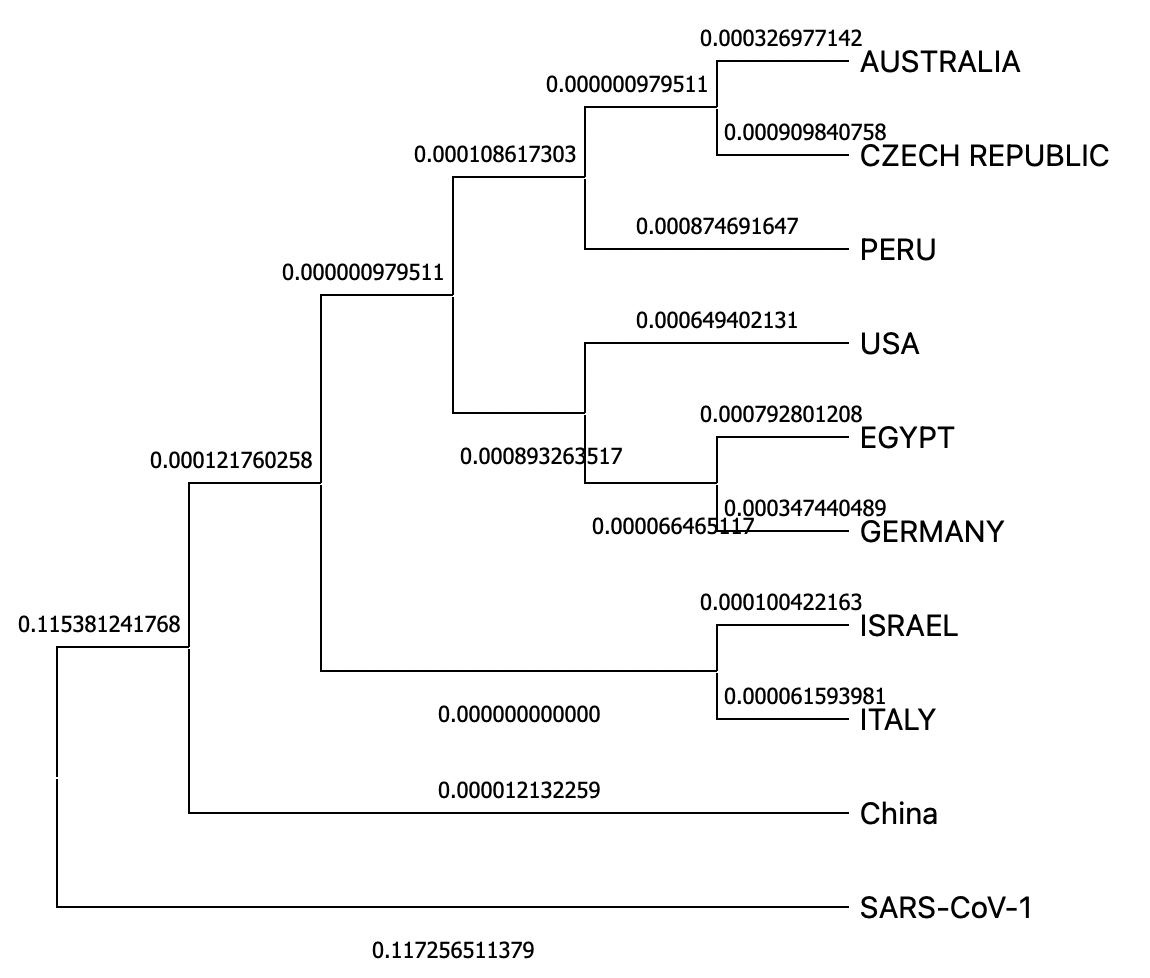
\includegraphics[scale=0.85]{images/ML.png}\\

Заметим, что в данном случае самый ближайший геном\\к SARS-CoV-1 - это Chine, а самый дальний - Germany и Egypt

\subparagraph{Maximum Parsimony\\}
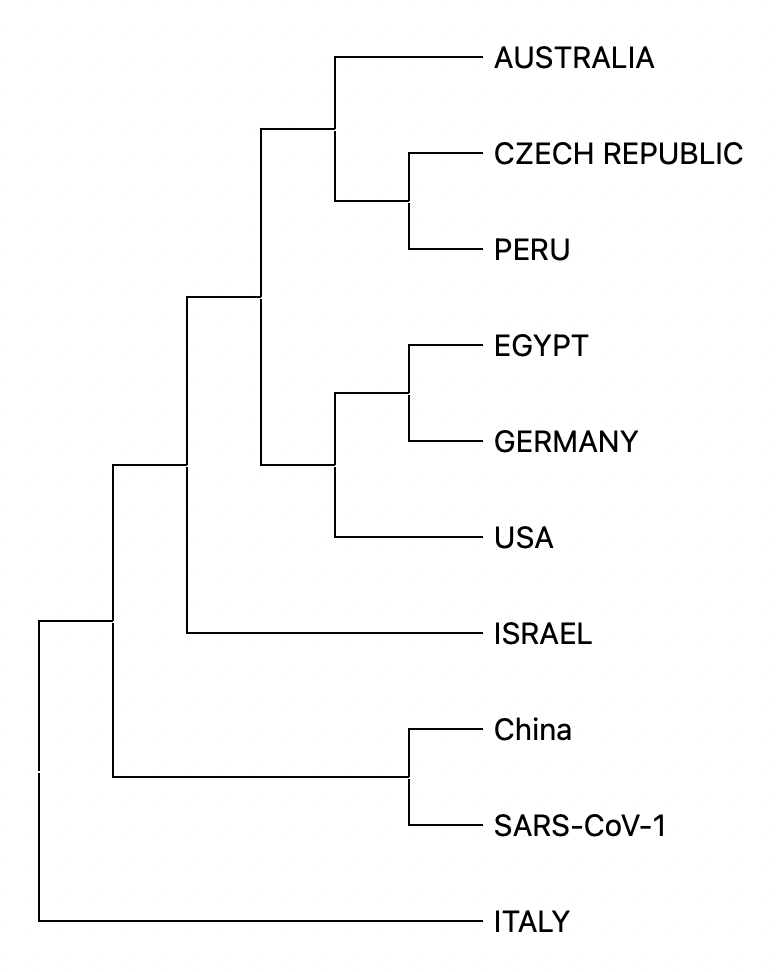
\includegraphics[scale=0.6]{images/MP.png}\\

Здесь мы не можем считать длины ветвей и искать самые ближние и самые дальние геномы к SARS-CoV-1, но по дереву видно, что оно соответвует тем результатам, которые были получены, анализируя предыдущие деревья. А именно, что самый ближайший геном к SARS-CoV-1 - это Chine, а самый дальний - Germany, Egypt \\


\subparagraph{Вывод:} человек, зараженный в Китае, переболел коронавирусом раньше всех, а человек из Германии и человек из Египта - позже всех. В целом такой результат неудивителен, так как я взял геном коронавируса из жителя Ухани (город, в котором началась эпидемия).

\newpage

\paragraph{Задание 2.} Теперь сравним последовательности геномов коронавируса из людей Китая и из Германии и найдем 5 мутаций. Возьмем координаты этих мутаций и определим, в каком гене они произошли.\\
Я нашел следующие 5 мутаций:\\
1) 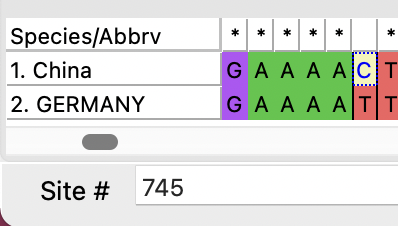
\includegraphics[scale=0.8]{images/Mismatch1.png}\\
2) 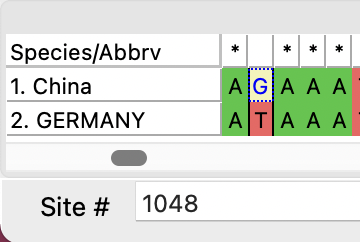
\includegraphics[scale=0.8]{images/Mismatch2.png}\\
3) 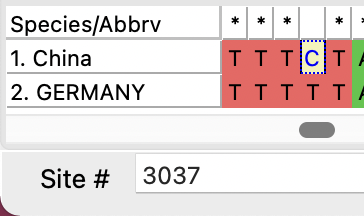
\includegraphics[scale=0.8]{images/Mismatch3.png}\\
4) 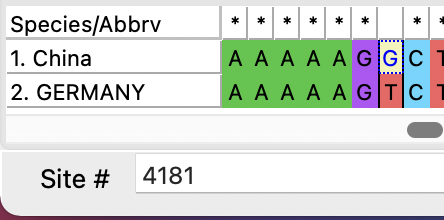
\includegraphics[scale=0.8]{images/Mismatch4.png}\\
5) 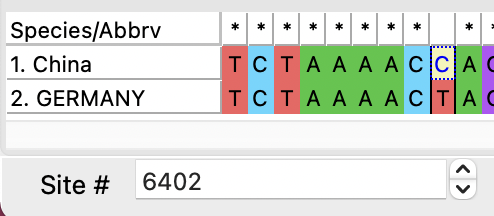
\includegraphics[scale=0.8]{images/Mismatch5.png}\\

\newpage

Теперь посмотрим на разметку генов:\\
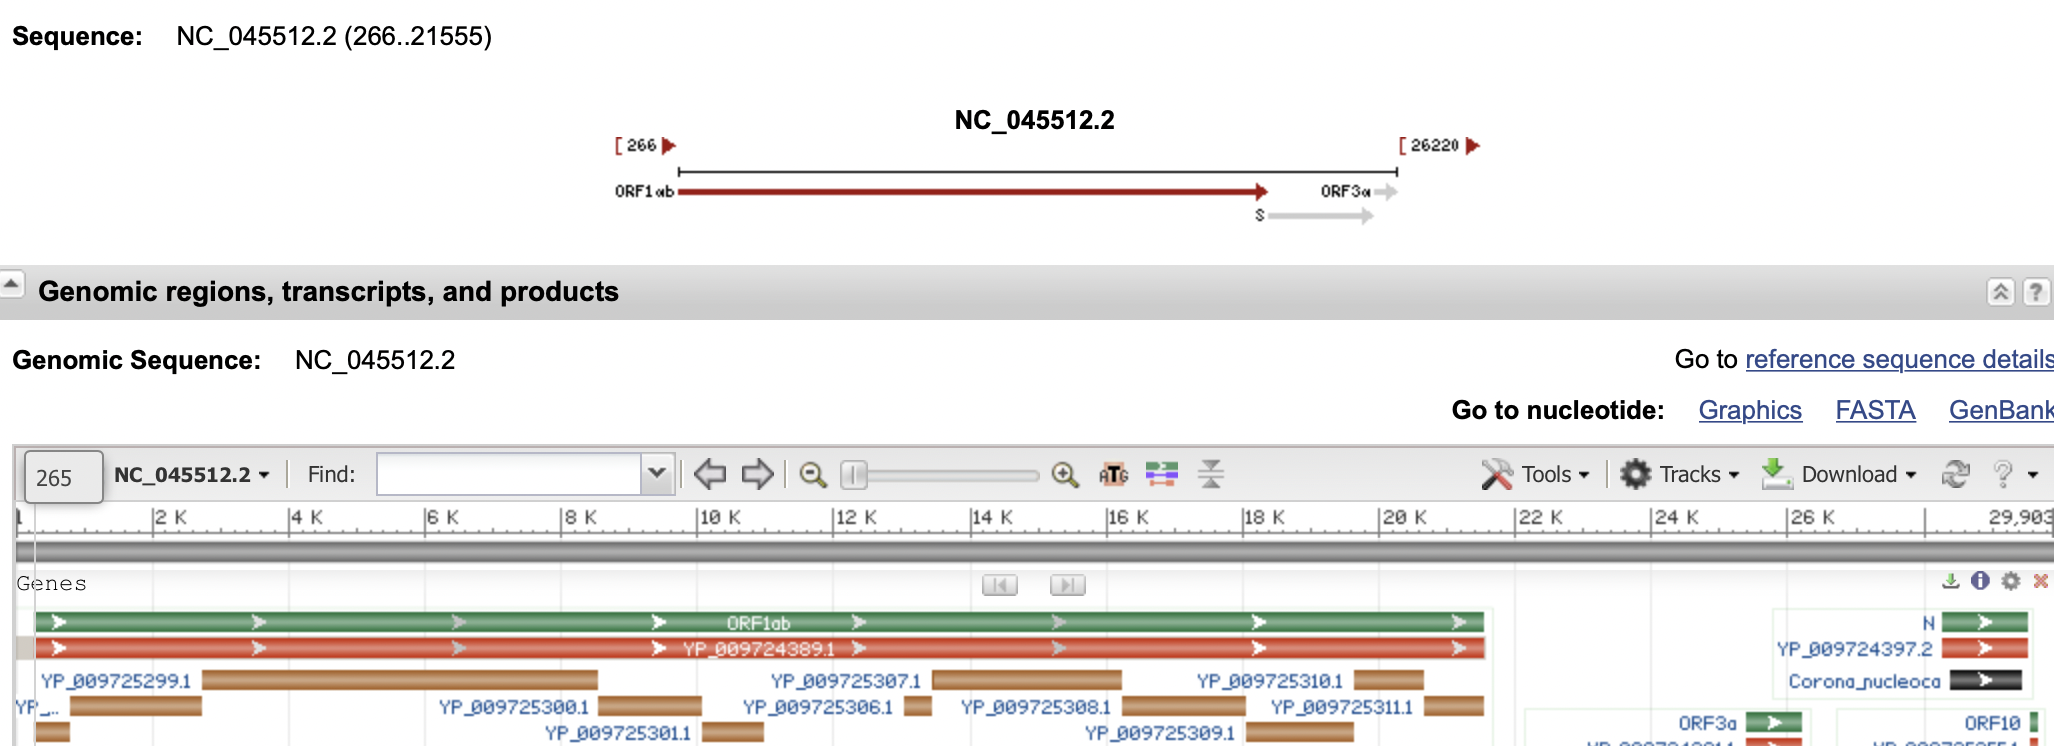
\includegraphics[scale=0.45]{images/razmetka.png}\\

Ясно, что найденные мной мутации произошли в гене ORF1ab.
\end{document}